\documentclass[color=usenames,dvipsnames]{beamer}\usepackage[]{graphicx}\usepackage[]{xcolor}
% maxwidth is the original width if it is less than linewidth
% otherwise use linewidth (to make sure the graphics do not exceed the margin)
\makeatletter
\def\maxwidth{ %
  \ifdim\Gin@nat@width>\linewidth
    \linewidth
  \else
    \Gin@nat@width
  \fi
}
\makeatother

\definecolor{fgcolor}{rgb}{0, 0, 0}
\newcommand{\hlnum}[1]{\textcolor[rgb]{0.69,0.494,0}{#1}}%
\newcommand{\hlstr}[1]{\textcolor[rgb]{0.749,0.012,0.012}{#1}}%
\newcommand{\hlcom}[1]{\textcolor[rgb]{0.514,0.506,0.514}{\textit{#1}}}%
\newcommand{\hlopt}[1]{\textcolor[rgb]{0,0,0}{#1}}%
\newcommand{\hlstd}[1]{\textcolor[rgb]{0,0,0}{#1}}%
\newcommand{\hlkwa}[1]{\textcolor[rgb]{0,0,0}{\textbf{#1}}}%
\newcommand{\hlkwb}[1]{\textcolor[rgb]{0,0.341,0.682}{#1}}%
\newcommand{\hlkwc}[1]{\textcolor[rgb]{0,0,0}{\textbf{#1}}}%
\newcommand{\hlkwd}[1]{\textcolor[rgb]{0.004,0.004,0.506}{#1}}%
\let\hlipl\hlkwb

\usepackage{framed}
\makeatletter
\newenvironment{kframe}{%
 \def\at@end@of@kframe{}%
 \ifinner\ifhmode%
  \def\at@end@of@kframe{\end{minipage}}%
  \begin{minipage}{\columnwidth}%
 \fi\fi%
 \def\FrameCommand##1{\hskip\@totalleftmargin \hskip-\fboxsep
 \colorbox{shadecolor}{##1}\hskip-\fboxsep
     % There is no \\@totalrightmargin, so:
     \hskip-\linewidth \hskip-\@totalleftmargin \hskip\columnwidth}%
 \MakeFramed {\advance\hsize-\width
   \@totalleftmargin\z@ \linewidth\hsize
   \@setminipage}}%
 {\par\unskip\endMakeFramed%
 \at@end@of@kframe}
\makeatother

\definecolor{shadecolor}{rgb}{.97, .97, .97}
\definecolor{messagecolor}{rgb}{0, 0, 0}
\definecolor{warningcolor}{rgb}{1, 0, 1}
\definecolor{errorcolor}{rgb}{1, 0, 0}
\newenvironment{knitrout}{}{} % an empty environment to be redefined in TeX

\usepackage{alltt}
%\documentclass[color=usenames,dvipsnames,handout]{beamer}

\usepackage[roman]{../lectures}
%\usepackage[sans]{../lectures}

\usepackage{booktabs}

\hypersetup{pdfpagemode=UseNone,pdfstartview={FitV}}


% Load function to compile and open PDF


% Compile and open PDF






%% New command for inline code that isn't to be evaluated
\definecolor{inlinecolor}{rgb}{0.878, 0.918, 0.933}
\newcommand{\inr}[1]{\colorbox{inlinecolor}{\texttt{#1}}}
\IfFileExists{upquote.sty}{\usepackage{upquote}}{}
\begin{document}




\begin{frame}[plain]
  \LARGE
%  \maketitle
  \centering
  {\LARGE Lecture 7 -- Multinomial $N$-mixture models: \\ simulation, fitting, and prediction} \\
  {\color{default} \rule{\textwidth}{0.1pt}}
  \vfill
  \large
  WILD(FISH) 8390 \\
%   Estimation of Fish and Wildlife Population Parameters \\
  Inference for Models of Fish and Wildlife Population Dynamics \\
  \vfill
  \large
  Richard Chandler \\
  University of Georgia \\
\end{frame}



\section{Overview}



\begin{frame}[plain]
  \frametitle{Outline}
  \Large
  \only<1>{\tableofcontents}%[hideallsubsections]}
  \only<2 | handout:0>{\tableofcontents[currentsection]}%,hideallsubsections]}
\end{frame}



\begin{frame}
  \frametitle{Overview}
  The objectives are the same as with binomial $N$-mixture models. %\\
%  \pause
%  \vfill
  We want to:
  \begin{itemize}
    \item Estimate abundance
    \item Model spatial variation in abundance/density
  \end{itemize}
  \pause
  \vfill
  The difference is that, instead of repeated count data at each site,
  we have data from sampling methods such as:
  \begin{itemize}
    \item<3-> Double observer sampling
    \item<3-> Removal sampling
    \item<3-> Mark-recapture
    \item<3-> Distance sampling
    \item<3-> And other methods that yield multinomial counts\dots
  \end{itemize}
\end{frame}




\begin{frame}
  \frametitle{Multinomial $N$-mixture model}
  \small
  State model (with Poisson assumption)
  \begin{gather*}
    \mathrm{log}(\lambda_i) = \beta_0 + \beta_1 {\color{blue} x_{i1}} +
    \beta_2 {\color{blue} x_{i2}} + \cdots \\
    N_i \sim \mathrm{Poisson}(\lambda_i)
  \end{gather*}
  \pause
  \vfill
  Observation model
  \begin{gather*}
    \mathrm{logit}(p_{ij}) = \alpha_0 + \alpha_1 {\color{blue} x_{i1}}
    + \alpha_2 {\color{Purple} w_{ij}} + \cdots \\
    \{y_{i1}, \dots, y_{iK}\}  \sim \mathrm{Multinomial}(N_i,
    \pi(p_{i1}, \dots, p_{iJ}))
  \end{gather*}
  \pause
%  \vfill
  \small
  Definitions \\
  \footnotesize
  $\lambda_i$ -- Expected value of abundance at site $i$ \\
  $N_i$ -- Realized value of abundance at site $i$ \\
  $p_{ij}$ -- Probability of detecting \alert{an individual} at site $i$ on occasion $j$ \\
  $\pi(p)$ -- Function mapping $J$ detection probs to
  $K$ multinomial cell probs \\
  $y_{ik}$ -- Multinomial count data (\alert{The final count is not observed!}) \\
%  \vfill
  $\color{blue} x_1$ and $\color{blue} x_2$ -- site covariates \hfill %\\
%  \vspace{12pt}
  $\color{Purple} w$ -- observation covariate
\end{frame}




\begin{frame}[fragile]
  \frametitle{The multinomial distribution}
  \small
  This is the first multivariate distribution we've covered. \\
  \[
    \{y_{1}, \dots, y_{K}\}  \sim \mathrm{Multinomial}(N, \{\pi_i, \dots, \pi_K\})
  \]
  \pause
%  \vfill
  The multinomial describes how $N$ objects are distributed among
  $K$ classes (also called bins, categories, etc\dots). \\
  \pause
  \vfill
  Imagine $N=20$ animals are studied for 1 year and there are 3
  possible ``fates'' with associated probabilities: \\
  $\Pr(\mathrm{survived})=0.5$, $\Pr(\mathrm{depredated})=0.3$, $\Pr(\mathrm{starved})=0.2$. \\
  \pause
  \vfill
  Here is one possible outcome:
  \vspace{-6pt}
\begin{knitrout}\footnotesize
\definecolor{shadecolor}{rgb}{0.878, 0.918, 0.933}\color{fgcolor}\begin{kframe}
\begin{alltt}
\hlstd{N} \hlkwb{<-} \hlnum{20}
\hlstd{pi} \hlkwb{<-} \hlkwd{c}\hlstd{(}\hlkwc{survived}\hlstd{=}\hlnum{0.5}\hlstd{,} \hlkwc{depredated}\hlstd{=}\hlnum{0.3}\hlstd{,} \hlkwc{starved}\hlstd{=}\hlnum{0.2}\hlstd{)}
\hlkwd{t}\hlstd{(}\hlkwd{rmultinom}\hlstd{(}\hlkwc{n}\hlstd{=}\hlnum{1}\hlstd{,} \hlkwc{size}\hlstd{=N,} \hlkwc{prob}\hlstd{=pi))}
\end{alltt}
\begin{verbatim}
##      survived depredated starved
## [1,]        8          9       3
\end{verbatim}
\end{kframe}
\end{knitrout}
  \pause
%  \vfill
  \centering
  Note: the probabilities must sum to 1 and the counts must sum to $N$. \\
\end{frame}



% \begin{frame}[fragile]
%   \frametitle{\normalsize Multinomial/Categorical vs Binomial/Bernoulli}
%   \centering
%   \fbox{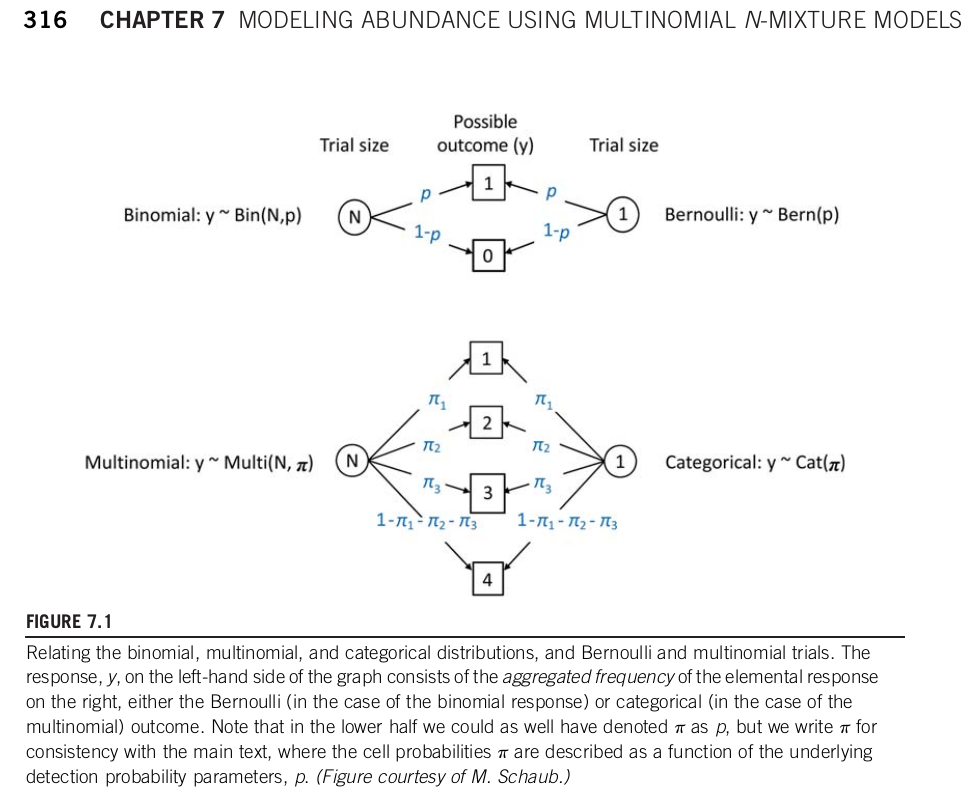
\includegraphics[width=0.85\textwidth]{figs/fig7-1}} \\
% \end{frame}



\begin{frame}
  \frametitle{Sampling methods}
  Benefits of the multinomial $N$-mixture model
  \begin{itemize}
    \item Can be applied to data from many sampling designs, simply by
      changing how the $\pi$ probabilities are computed. %\\
    \item Precision is typically better than binomial $N$-mixture
      models because there's more information in the data
  \end{itemize}
  \pause
  \vfill
  Removal sampling %\\
  \[
    {\pi(p)} = \{p, (1-p)p, (1-p)^2p, \dots, (1-p)^{K-1}p, (1-p)^K\}
  \]
  \pause %\vfill
  Double observer (\alert{independent observers})
  \[
    {\pi(p)} = \{p_1(1-p_2), (1-p_1)p_2, p_1p_2, (1-p_1)(1-p_2)\}
  \]
  \pause %\vfill
  Double observer (\alert{dependent observers})
  \[
    {\pi(p)} = \{p_1, (1-p_1)p_2, (1-p_1)(1-p_2)\}
  \]
\end{frame}




%\section{Simulation}

\section{Removal sampling}

\subsection{Likelihood-based methods}

\begin{frame}
  \frametitle{Outline}
  \Large
%  \tableofcontents[currentsection,currentsubsection]
  \tableofcontents[currentsection]
\end{frame}



\begin{frame}
  \frametitle{Removal sampling}
  \small
  Removal sampling is often used in electrofishing studies. \\
  \pause
  \vfill
  A stream section is surveyed $J$ times, fish are removed on each
  ``pass'', and the rate of removal tells us about capture
  probability.  
  \pause
  \vfill
  Definitions
  \begin{itemize}
    \setlength\itemsep{1pt}
    \item $y_{ij}$ -- number of individuals removed at site $i$ on pass $j$
    \item $p$ -- probability of catching an individual on a single pass
  \end{itemize}
  \pause \vfill
  \footnotesize
  \begin{tabular}{lc}
    \hline
    \centering
    Description                       & Multinomial cell probability \\
    \hline
    Pr(first captured on first pass)  & $\pi_1 = p$                  \\
    Pr(first captured on second pass) & $\pi_2 = (1-p)p$             \\
    Pr(first captured on third pass)  & $\pi_3 = (1-p)(1-p)p$        \\
    {\centering $\cdots$}             & $\cdots$                     \\
    Pr(first captured on pass $J$)    & $\pi_J = (1-p)^{J-1}p$       \\
    Pr(not captured)                  & $\pi_{J+1} = (1-p)^J$          \\
    \hline
  \end{tabular}
\end{frame}







\begin{frame}[fragile]
  \frametitle{Simulating removal data, no covariates}
  \small
  Abundance
\begin{knitrout}\scriptsize
\definecolor{shadecolor}{rgb}{0.878, 0.918, 0.933}\color{fgcolor}\begin{kframe}
\begin{alltt}
\hlstd{nSites} \hlkwb{<-} \hlnum{100}
\hlstd{lambda1} \hlkwb{<-} \hlnum{4.6}  \hlcom{## Expected value of N}
\hlstd{N1} \hlkwb{<-} \hlkwd{rpois}\hlstd{(}\hlkwc{n}\hlstd{=nSites,} \hlkwc{lambda}\hlstd{=lambda1)}
\end{alltt}
\end{kframe}
\end{knitrout}
% \item
  \pause
  \vfill
  Capture probability and multinomial counts%, including individuals
%  \alert{not} detected
\begin{knitrout}\scriptsize
\definecolor{shadecolor}{rgb}{0.878, 0.918, 0.933}\color{fgcolor}\begin{kframe}
\begin{alltt}
\hlstd{nPasses} \hlkwb{<-} \hlnum{3}
\hlstd{K} \hlkwb{<-} \hlstd{nPasses}\hlopt{+}\hlnum{1}  \hlcom{# multinomial cells}
\hlstd{p1} \hlkwb{<-} \hlnum{0.4}
\hlstd{pi1} \hlkwb{<-} \hlkwd{c}\hlstd{(p1, (}\hlnum{1}\hlopt{-}\hlstd{p1)}\hlopt{*}\hlstd{p1, (}\hlnum{1}\hlopt{-}\hlstd{p1)}\hlopt{*}\hlstd{(}\hlnum{1}\hlopt{-}\hlstd{p1)}\hlopt{*}\hlstd{p1, (}\hlnum{1}\hlopt{-}\hlstd{p1)}\hlopt{^}\hlnum{3}\hlstd{)}
\hlstd{y1.all} \hlkwb{<-} \hlkwd{matrix}\hlstd{(}\hlnum{NA}\hlstd{,} \hlkwc{nrow}\hlstd{=nSites,} \hlkwc{ncol}\hlstd{=K)}
\hlkwa{for}\hlstd{(i} \hlkwa{in} \hlnum{1}\hlopt{:}\hlstd{nSites) \{}
    \hlstd{y1.all[i,]} \hlkwb{<-} \hlkwd{rmultinom}\hlstd{(}\hlkwc{n}\hlstd{=}\hlnum{1}\hlstd{,} \hlkwc{size}\hlstd{=N1[i],} \hlkwc{prob}\hlstd{=pi1)    \}}
\end{alltt}
\end{kframe}
\end{knitrout}
%\end{enumerate}
  \pause
  \vfill
  Discard final column of individuals not detected
\begin{knitrout}\scriptsize
\definecolor{shadecolor}{rgb}{0.878, 0.918, 0.933}\color{fgcolor}\begin{kframe}
\begin{alltt}
\hlstd{y1} \hlkwb{<-} \hlstd{y1.all[,}\hlopt{-}\hlstd{K]}
\hlkwd{head}\hlstd{(y1,} \hlkwc{n}\hlstd{=}\hlnum{3}\hlstd{)}
\end{alltt}
\begin{verbatim}
##      [,1] [,2] [,3]
## [1,]    0    1    1
## [2,]    1    2    0
## [3,]    2    0    1
\end{verbatim}
\end{kframe}
\end{knitrout}
\end{frame}



\begin{frame}[fragile]
  \frametitle{Simulated removal data}
\begin{knitrout}
\definecolor{shadecolor}{rgb}{0.878, 0.918, 0.933}\color{fgcolor}\begin{table}

\begin{tabular}{lrrr}
\toprule
  & Pass 1 & Pass 2 & Pass 3\\
\midrule
Site 1 & 0 & 1 & 1\\
Site 2 & 1 & 2 & 0\\
Site 3 & 2 & 0 & 1\\
Site 4 & 2 & 0 & 0\\
Site 5 & 7 & 1 & 1\\
\addlinespace
Site 6 & 2 & 1 & 0\\
Site 7 & 3 & 2 & 1\\
Site 8 & 2 & 0 & 0\\
Site 9 & 4 & 0 & 1\\
Site 10 & 0 & 1 & 0\\
\bottomrule
\end{tabular}
\end{table}

\end{knitrout}
\end{frame}


\begin{frame}[fragile]
  \frametitle{Removal model, covariates}
  \small
  Covariates
  \vspace{-6pt}
\begin{knitrout}\scriptsize
\definecolor{shadecolor}{rgb}{0.878, 0.918, 0.933}\color{fgcolor}\begin{kframe}
\begin{alltt}
\hlstd{streamDepth} \hlkwb{<-} \hlkwd{rnorm}\hlstd{(nSites)}
\end{alltt}
\end{kframe}
\end{knitrout}
% \item
\vfill
  Coefficients, $\lambda$, and $p$
  \vspace{-6pt}
\begin{knitrout}\scriptsize
\definecolor{shadecolor}{rgb}{0.878, 0.918, 0.933}\color{fgcolor}\begin{kframe}
\begin{alltt}
\hlstd{beta0} \hlkwb{<-} \hlnum{1}\hlstd{; beta1} \hlkwb{<-} \hlnum{0.5}
\hlstd{lambda2} \hlkwb{<-} \hlkwd{exp}\hlstd{(beta0} \hlopt{+} \hlstd{beta1}\hlopt{*}\hlstd{streamDepth)}
\hlstd{alpha0} \hlkwb{<-} \hlnum{0}\hlstd{; alpha1} \hlkwb{<-} \hlopt{-}\hlnum{1}
\hlstd{p2} \hlkwb{<-} \hlkwd{plogis}\hlstd{(alpha0} \hlopt{+} \hlstd{alpha1}\hlopt{*}\hlstd{streamDepth)}
\end{alltt}
\end{kframe}
\end{knitrout}
% \item
\vfill
  Simulate abundance and removal data
  \vspace{-6pt}
\begin{knitrout}\scriptsize
\definecolor{shadecolor}{rgb}{0.878, 0.918, 0.933}\color{fgcolor}\begin{kframe}
\begin{alltt}
\hlstd{N2} \hlkwb{<-} \hlkwd{rpois}\hlstd{(nSites,} \hlkwc{lambda}\hlstd{=lambda2)}         \hlcom{## local abundance }
\hlstd{y2.all} \hlkwb{<-} \hlstd{pi2} \hlkwb{<-} \hlkwd{matrix}\hlstd{(}\hlnum{NA}\hlstd{,} \hlkwc{nrow}\hlstd{=nSites,} \hlkwc{ncol}\hlstd{=K)}
\hlkwa{for}\hlstd{(i} \hlkwa{in} \hlnum{1}\hlopt{:}\hlstd{nSites) \{}
    \hlstd{pi2[i,]} \hlkwb{<-} \hlkwd{c}\hlstd{(p2[i], (}\hlnum{1}\hlopt{-}\hlstd{p2[i])}\hlopt{*}\hlstd{p2[i], (}\hlnum{1}\hlopt{-}\hlstd{p2[i])}\hlopt{^}\hlnum{2}\hlopt{*}\hlstd{p2[i], (}\hlnum{1}\hlopt{-}\hlstd{p2[i])}\hlopt{^}\hlnum{3}\hlstd{)}
    \hlstd{y2.all[i,]} \hlkwb{<-} \hlkwd{rmultinom}\hlstd{(}\hlkwc{n}\hlstd{=}\hlnum{1}\hlstd{,} \hlkwc{size}\hlstd{=N2[i],} \hlkwc{prob}\hlstd{=pi2[i,])}
\hlstd{\}}
\hlstd{y2} \hlkwb{<-} \hlstd{y2.all[,}\hlopt{-}\hlstd{K]} \hlcom{## Discard final column... individuals not detected}
\end{alltt}
\end{kframe}
\end{knitrout}
%\end{enumerate}
\end{frame}




\begin{frame}[fragile]
  \frametitle{Simulated data}
  \begin{columns}
    \begin{column}{0.4\textwidth}
      \small
      Observations
%      \tiny
  \vspace{-6pt}
\begin{knitrout}\scriptsize
\definecolor{shadecolor}{rgb}{0.878, 0.918, 0.933}\color{fgcolor}\begin{kframe}
\begin{alltt}
\hlstd{y2[}\hlnum{1}\hlopt{:}\hlnum{19}\hlstd{,]}
\end{alltt}
\begin{verbatim}
##       [,1] [,2] [,3]
##  [1,]    1    0    0
##  [2,]    0    0    0
##  [3,]    1    0    0
##  [4,]    1    1    0
##  [5,]    0    0    0
##  [6,]    0    0    0
##  [7,]    0    1    0
##  [8,]    1    0    0
##  [9,]    1    2    0
## [10,]    2    0    0
## [11,]    3    0    0
## [12,]    2    0    0
## [13,]    1    2    0
## [14,]    0    0    0
## [15,]    3    2    1
## [16,]    0    0    0
## [17,]    0    1    0
## [18,]    4    1    1
## [19,]    1    0    0
\end{verbatim}
\end{kframe}
\end{knitrout}
  \end{column}
  \begin{column}{0.6\textwidth}
%    \pause
%    \scriptsize
    {\centering Summary stats \\}
    \vspace{24pt}
    \small
  \pause
  \vfill
  \small
  Captures on each pass
  \vspace{-6pt}
\begin{knitrout}\scriptsize
\definecolor{shadecolor}{rgb}{0.878, 0.918, 0.933}\color{fgcolor}\begin{kframe}
\begin{alltt}
\hlkwd{colSums}\hlstd{(y2)}
\end{alltt}
\begin{verbatim}
## [1] 119  62  36
\end{verbatim}
\end{kframe}
\end{knitrout}
  \pause
  \vfill
  Naive abundance
  \vspace{-6pt}
\begin{knitrout}\scriptsize
\definecolor{shadecolor}{rgb}{0.878, 0.918, 0.933}\color{fgcolor}\begin{kframe}
\begin{alltt}
\hlkwd{sum}\hlstd{(y2)}
\end{alltt}
\begin{verbatim}
## [1] 217
\end{verbatim}
\end{kframe}
\end{knitrout}

  \end{column}
  \end{columns}
\end{frame}









%\section{Prediction}



% \begin{frame}
%   \frametitle{Outline}
%   \Large
%   \tableofcontents[currentsection]
% \end{frame}






\begin{frame}[fragile]
  \frametitle{Prepare data in `unmarked'}
  \small
\begin{knitrout}\tiny
\definecolor{shadecolor}{rgb}{0.878, 0.918, 0.933}\color{fgcolor}\begin{kframe}
\begin{alltt}
\hlstd{umf} \hlkwb{<-} \hlkwd{unmarkedFrameMPois}\hlstd{(}\hlkwc{y}\hlstd{=y2,} \hlkwc{siteCovs}\hlstd{=}\hlkwd{data.frame}\hlstd{(streamDepth),} \hlkwc{type}\hlstd{=}\hlstr{"removal"}\hlstd{)}
\end{alltt}
\end{kframe}
\end{knitrout}
\pause
\begin{knitrout}\scriptsize
\definecolor{shadecolor}{rgb}{0.878, 0.918, 0.933}\color{fgcolor}\begin{kframe}
\begin{alltt}
\hlkwd{summary}\hlstd{(umf)}
\end{alltt}
\begin{verbatim}
## unmarkedFrame Object
## 
## 100 sites
## Maximum number of observations per site: 3 
## Mean number of observations per site: 3 
## Sites with at least one detection: 89 
## 
## Tabulation of y observations:
##   0   1   2   3   4 
## 153  98  32  13   4 
## 
## Site-level covariates:
##   streamDepth       
##  Min.   :-2.328970  
##  1st Qu.:-0.954293  
##  Median : 0.001277  
##  Mean   :-0.120419  
##  3rd Qu.: 0.569628  
##  Max.   : 2.610328
\end{verbatim}
\end{kframe}
\end{knitrout}
\end{frame}


% > fm <- multinomPois(~temp ~forest, umf)    

% error: Mat::operator(): index out of bounds
% terminate called after throwing an instance of 'std::logic_error'
%   what():  Mat::operator(): index out of bounds


\begin{frame}[fragile]
  \frametitle{Fit the model}
  \footnotesize
  \inr{multinomPois} has similar arguments as \inr{occu} and
  \inr{pcount}. 
\begin{knitrout}\tiny
\definecolor{shadecolor}{rgb}{0.878, 0.918, 0.933}\color{fgcolor}\begin{kframe}
\begin{alltt}
\hlstd{fm} \hlkwb{<-} \hlkwd{multinomPois}\hlstd{(}\hlopt{~}\hlstd{streamDepth} \hlopt{~}\hlstd{streamDepth, umf)}
\hlstd{fm}
\end{alltt}
\begin{verbatim}
## 
## Call:
## multinomPois(formula = ~streamDepth ~ streamDepth, data = umf)
## 
## Abundance:
##             Estimate    SE     z  P(>|z|)
## (Intercept)     1.04 0.101 10.31 6.29e-25
## streamDepth     0.56 0.115  4.89 1.02e-06
## 
## Detection:
##             Estimate    SE      z  P(>|z|)
## (Intercept)  -0.0426 0.214 -0.199 8.42e-01
## streamDepth  -1.0084 0.171 -5.902 3.59e-09
## 
## AIC: 603.3294
\end{verbatim}
\end{kframe}
\end{knitrout}
\pause
\vfill
Compare to actual parameter values:
\vspace{-6pt}
\begin{knitrout}\tiny
\definecolor{shadecolor}{rgb}{0.878, 0.918, 0.933}\color{fgcolor}\begin{kframe}
\begin{alltt}
\hlkwd{c}\hlstd{(}\hlkwc{beta0}\hlstd{=beta0,} \hlkwc{beta1}\hlstd{=beta1);} \hlkwd{c}\hlstd{(}\hlkwc{alpha0}\hlstd{=alpha0,} \hlkwc{alpha1}\hlstd{=alpha1)}
\end{alltt}
\begin{verbatim}
## beta0 beta1 
##   1.0   0.5
## alpha0 alpha1 
##      0     -1
\end{verbatim}
\end{kframe}
\end{knitrout}
\end{frame}





\begin{frame}[fragile]
  \frametitle{\normalsize Empirical Bayes -- Site-level abundance}
\begin{knitrout}\scriptsize
\definecolor{shadecolor}{rgb}{0.878, 0.918, 0.933}\color{fgcolor}\begin{kframe}
\begin{alltt}
\hlstd{re} \hlkwb{<-} \hlkwd{ranef}\hlstd{(fm,} \hlkwc{K}\hlstd{=}\hlnum{15}\hlstd{)}
\hlkwd{plot}\hlstd{(re,} \hlkwc{layout}\hlstd{=}\hlkwd{c}\hlstd{(}\hlnum{4}\hlstd{,}\hlnum{3}\hlstd{),} \hlkwc{subset}\hlstd{=site}\hlopt\hlnum{1}\hlopt{:}\hlnum{12}\hlstd{,} \hlkwc{xlim}\hlstd{=}\hlkwd{c}\hlstd{(}\hlopt{-}\hlnum{1}\hlstd{,} \hlnum{11}\hlstd{),} \hlkwc{lwd}\hlstd{=}\hlnum{5}\hlstd{)}
\end{alltt}
\end{kframe}

{\centering \includegraphics[width=0.8\linewidth]{figure/ranef-1} 

}


\end{knitrout}
\end{frame}





\begin{frame}[fragile]
  \frametitle{Total abundance (in surveyed region)}
\begin{knitrout}\scriptsize
\definecolor{shadecolor}{rgb}{0.878, 0.918, 0.933}\color{fgcolor}\begin{kframe}
\begin{alltt}
\hlstd{N.total.post} \hlkwb{<-} \hlkwd{predict}\hlstd{(re,} \hlkwc{func}\hlstd{=sum,} \hlkwc{nsim}\hlstd{=}\hlnum{1000}\hlstd{)}
\hlkwd{hist}\hlstd{(N.total.post,} \hlkwc{freq}\hlstd{=}\hlnum{FALSE}\hlstd{,} \hlkwc{main}\hlstd{=}\hlstr{""}\hlstd{,} \hlkwc{xlab}\hlstd{=}\hlstr{"N total"}\hlstd{,} \hlkwc{ylab}\hlstd{=}\hlstr{"Probability"}\hlstd{)}
\end{alltt}
\end{kframe}

{\centering \includegraphics[width=0.6\linewidth]{figure/Ntotal-1} 

}


\end{knitrout}
\end{frame}






\begin{frame}[fragile]
  \frametitle{Prediction in `unmarked'}
  \small
  Create \texttt{data.frame} with prediction covariates. 
  \vspace{-6pt}
\begin{knitrout}\footnotesize
\definecolor{shadecolor}{rgb}{0.878, 0.918, 0.933}\color{fgcolor}\begin{kframe}
\begin{alltt}
\hlstd{pred.data} \hlkwb{<-} \hlkwd{data.frame}\hlstd{(}\hlkwc{streamDepth}\hlstd{=}\hlkwd{seq}\hlstd{(}\hlopt{-}\hlnum{3}\hlstd{,} \hlnum{3}\hlstd{,} \hlkwc{length}\hlstd{=}\hlnum{20}\hlstd{))}
\end{alltt}
\end{kframe}
\end{knitrout}
\pause
\vfill
Get predictions of $\lambda$ for each row of prediction data.
  \vspace{-6pt}
\begin{knitrout}\footnotesize
\definecolor{shadecolor}{rgb}{0.878, 0.918, 0.933}\color{fgcolor}\begin{kframe}
\begin{alltt}
\hlstd{lambda.pred} \hlkwb{<-} \hlkwd{predict}\hlstd{(fm,} \hlkwc{newdata}\hlstd{=pred.data,}
                       \hlkwc{type}\hlstd{=}\hlstr{'state'}\hlstd{,} \hlkwc{append}\hlstd{=}\hlnum{TRUE}\hlstd{)}
\end{alltt}
\end{kframe}
\end{knitrout}
\pause
\vfill
  View $\lambda$ predictions
  \vspace{-6pt}
\begin{knitrout}\footnotesize
\definecolor{shadecolor}{rgb}{0.878, 0.918, 0.933}\color{fgcolor}\begin{kframe}
\begin{alltt}
\hlkwd{print}\hlstd{(}\hlkwd{head}\hlstd{(lambda.pred),} \hlkwc{digits}\hlstd{=}\hlnum{2}\hlstd{)}
\end{alltt}
\begin{verbatim}
##   Predicted   SE lower upper streamDepth
## 1      0.53 0.16  0.29  0.97        -3.0
## 2      0.63 0.17  0.37  1.08        -2.7
## 3      0.75 0.18  0.47  1.20        -2.4
## 4      0.90 0.19  0.60  1.35        -2.1
## 5      1.07 0.19  0.76  1.51        -1.7
## 6      1.28 0.18  0.97  1.70        -1.4
\end{verbatim}
\end{kframe}
\end{knitrout}
\end{frame}





\begin{frame}[fragile]
  \frametitle{Prediction in `unmarked'}
\begin{knitrout}\tiny
\definecolor{shadecolor}{rgb}{0.878, 0.918, 0.933}\color{fgcolor}\begin{kframe}
\begin{alltt}
\hlkwd{plot}\hlstd{(Predicted} \hlopt{~} \hlstd{streamDepth, lambda.pred,} \hlkwc{ylab}\hlstd{=}\hlstr{"Expected value of abundance"}\hlstd{,}
     \hlkwc{ylim}\hlstd{=}\hlkwd{c}\hlstd{(}\hlnum{0}\hlstd{,}\hlnum{20}\hlstd{),} \hlkwc{xlab}\hlstd{=}\hlstr{"Stream depth"}\hlstd{,} \hlkwc{type}\hlstd{=}\hlstr{"l"}\hlstd{,} \hlkwc{lwd}\hlstd{=}\hlnum{2}\hlstd{)}
\hlkwd{lines}\hlstd{(lower} \hlopt{~} \hlstd{streamDepth, lambda.pred,} \hlkwc{col}\hlstd{=}\hlstr{"grey"}\hlstd{)}
\hlkwd{lines}\hlstd{(upper} \hlopt{~} \hlstd{streamDepth, lambda.pred,} \hlkwc{col}\hlstd{=}\hlstr{"grey"}\hlstd{)}
\hlkwd{points}\hlstd{(}\hlkwd{rowSums}\hlstd{(y2)}\hlopt{~}\hlstd{streamDepth)}
\hlkwd{lines}\hlstd{(}\hlkwd{lowess}\hlstd{(}\hlkwd{rowSums}\hlstd{(y2)}\hlopt{~}\hlstd{streamDepth),} \hlkwc{col}\hlstd{=}\hlstr{"blue"}\hlstd{,} \hlkwc{lwd}\hlstd{=}\hlnum{2}\hlstd{)}  \hlcom{## Loess line for fun (it's way off)}
\end{alltt}
\end{kframe}

{\centering \includegraphics[width=0.8\linewidth]{figure/pred-lam2-1} 

}


\end{knitrout}
\end{frame}







\begin{frame}[fragile]
  \frametitle{In-class exercise}
  % \small
  % \begin{enumerate}
  %   \item Predict
  %   \end{enumerate}
  %   \centering
%  \large
  Do the following using the fitted removal model above:
  \begin{enumerate}
    \normalsize
    \item Predict $p$ when \verb+streamDepth=-1+
    \item Use the prediction of $p$ to compute $\pi_1, \pi_2, \pi_3, \pi_4$
  \end{enumerate}
\end{frame}


\subsection{Bayesian methods}


\begin{frame}
  \frametitle{Outline}
  \Large
  \tableofcontents[currentsection,currentsubsection]
\end{frame}


\begin{frame}
  \frametitle{Bayesian multinomial $N$-mixture models}
  There are several equivalent formulations of the multinomial, some
  of which that we can exploit to fit the model in JAGS. \\
  
  \begin{itemize}
    \item Conditional-on-$N$, missing $y_{iK}$ (Not possible in JAGS)
    \item Conditional-on-$N$, conditional on $n_i=\sum_{k=1}^{K-1} y_{i,k}$
    \item Conditional-on-$N$, sequential binomial
    \item Marginalized $N$
  \end{itemize}
  \pause
  \vfill
  These are just probability tricks that can affect MCMC
  performance. See AHM I for details. Here, we will focus on the second
  option. \\ 
\end{frame}




% \begin{frame}[fragile]
%   \frametitle{Conditional-on-$N$, missing $y_k$}
% \end{frame}





% \begin{frame}[fragile]
%   \frametitle{Conditional-on-$N$, missing $y_k$}
%   \footnotesize
%   Under this formulation, we view the final multinomial cell
%   (corresponding to individuals not detected) as missing data. \\
%   \pause
%   \vfill
%   Unfortunately, this won't work in JAGS because it doesn't allow
%   missing values in multinomial outcomes.
%   \pause
% <<bugs-removal1,size='tiny',echo=FALSE,comment='',background='lightblue'>>=
% writeLines(readLines("removal-mod1.jag"))
% @
% <<jagsUI,include=FALSE>>=
% library(jagsUI)
% @ 
% \end{frame}





\begin{frame}[fragile]
  \frametitle{\normalsize Conditional-on-$N$ and $n_i=\sum_{k=1}^{K-1} y_{i,k}$}
  % Rather than treating the final multinomial cell as missing data:
  % \[
  %   \{y_{i,1}, \dots, y_{i,K-1}, \mathtt{\color{red} NA}\} \sim
  %   \mathrm{Multinomial}(N_i, \{\pi_{i,1}, \dots, \pi_{i,K-1}, \pi_{i,K}\})
  % \]
  % \pause
  % \vfill
  We can break the problem down into two steps by conditioning on
  $n_i$, the number of individuals captured at site $i$:
  \small
  \begin{gather*}
    n_i \sim \mathrm{Bin}(N_i, 1-\pi_K) \\
    \{y_{i,1}, \dots, y_{i,K-1}\} \sim \mathrm{Multinomial}(n_i,
    \{\pi_{i,1}, \dots, \pi_{i,K-1}\}/(1-\pi_K))
  \end{gather*}
  \pause
  \vfill
  Note that the modified cell probabilities still sum to 1. 
\end{frame}



\begin{frame}[fragile]
  \frametitle{\normalsize Conditional-on-$N$ and $n_i=\sum_{k=1}^{K-1} y_{i,k}$}
\vspace{-3pt}
\begin{knitrout}\scriptsize
\definecolor{shadecolor}{rgb}{0.678, 0.847, 0.902}\color{fgcolor}\begin{kframe}
\begin{verbatim}
model {

lambda.intercept ~ dunif(0, 5)
beta0 <- log(lambda.intercept)
beta1 ~ dnorm(0, 0.5)

alpha0 ~ dnorm(0, 0.5)  
alpha1 ~ dnorm(0, 0.5)

for(i in 1:nSites) {
  log(lambda[i]) <- beta0 + beta1*streamDepth[i]
  N[i] ~ dpois(lambda[i])         # Latent local abundance
  logit(p[i]) <- alpha0 + alpha1*streamDepth[i]
  pi[i,1] <- p[i]               ## Pr(first captured in first pass)
  pi[i,2] <- (1-p[i])*p[i]      ## Pr(first captured in second pass)
  pi[i,3] <- (1-p[i])^2*p[i]    ## Pr(first captured in third pass)
  pi[i,4] <- (1-p[i])^3         ## Pr(not captured)
  n[i] ~ dbin(1-pi[i,4], N[i])  ## nCaptured at site i
  y[i,1:3] ~ dmulti(pi[i,1:3]/(1-pi[i,4]), n[i])
}

totalAbundance <- sum(N[1:nSites])

}
\end{verbatim}
\end{kframe}
\end{knitrout}
\end{frame}





\begin{frame}[fragile]
  \frametitle{Data, inits, and parameters}
  Put data in a named list
  \vspace{-12pt}
\begin{knitrout}\small
\definecolor{shadecolor}{rgb}{0.878, 0.918, 0.933}\color{fgcolor}\begin{kframe}
\begin{alltt}
\hlstd{jags.data.rem2} \hlkwb{<-} \hlkwd{list}\hlstd{(}\hlkwc{y}\hlstd{=y2,} \hlkwc{n}\hlstd{=}\hlkwd{rowSums}\hlstd{(y2),}
                       \hlkwc{streamDepth}\hlstd{=streamDepth,}
                       \hlkwc{nSites}\hlstd{=nSites,} \hlkwc{nPasses}\hlstd{=nPasses)}
\end{alltt}
\end{kframe}
\end{knitrout}
\pause
\vfill
  Initial values
  \vspace{-12pt}
\begin{knitrout}\small
\definecolor{shadecolor}{rgb}{0.878, 0.918, 0.933}\color{fgcolor}\begin{kframe}
\begin{alltt}
\hlstd{jags.inits.rem} \hlkwb{<-} \hlkwa{function}\hlstd{() \{}
    \hlkwd{list}\hlstd{(}\hlkwc{lambda.intercept}\hlstd{=}\hlkwd{runif}\hlstd{(}\hlnum{1}\hlstd{),} \hlkwc{alpha0}\hlstd{=}\hlkwd{rnorm}\hlstd{(}\hlnum{1}\hlstd{),}
         \hlkwc{N}\hlstd{=}\hlkwd{rowSums}\hlstd{(y2)}\hlopt{+}\hlkwd{rpois}\hlstd{(}\hlkwd{nrow}\hlstd{(y2),} \hlnum{2}\hlstd{))}
\hlstd{\}}
\end{alltt}
\end{kframe}
\end{knitrout}
\pause
\vfill
  Parameters to monitor
  \vspace{-12pt}
\begin{knitrout}\small
\definecolor{shadecolor}{rgb}{0.878, 0.918, 0.933}\color{fgcolor}\begin{kframe}
\begin{alltt}
\hlstd{jags.pars.rem} \hlkwb{<-} \hlkwd{c}\hlstd{(}\hlstr{"beta0"}\hlstd{,} \hlstr{"beta1"}\hlstd{,}
                   \hlstr{"alpha0"}\hlstd{,} \hlstr{"alpha1"}\hlstd{,} \hlstr{"totalAbundance"}\hlstd{)}
\end{alltt}
\end{kframe}
\end{knitrout}
\end{frame}





\begin{frame}[fragile]
  \frametitle{MCMC}
  \small
\begin{knitrout}\tiny
\definecolor{shadecolor}{rgb}{0.878, 0.918, 0.933}\color{fgcolor}\begin{kframe}
\begin{alltt}
\hlkwd{library}\hlstd{(jagsUI);} \hlkwd{library}\hlstd{(coda)}
\hlstd{jags.post.rem2} \hlkwb{<-} \hlkwd{jags.basic}\hlstd{(}\hlkwc{data}\hlstd{=jags.data.rem2,} \hlkwc{inits}\hlstd{=jags.inits.rem,}
                             \hlkwc{parameters.to.save}\hlstd{=jags.pars.rem,} \hlkwc{model.file}\hlstd{=}\hlstr{"removal-mod2.jag"}\hlstd{,}
                             \hlkwc{n.chains}\hlstd{=}\hlnum{3}\hlstd{,} \hlkwc{n.adapt}\hlstd{=}\hlnum{100}\hlstd{,} \hlkwc{n.burnin}\hlstd{=}\hlnum{0}\hlstd{,} \hlkwc{n.iter}\hlstd{=}\hlnum{2000}\hlstd{,} \hlkwc{parallel}\hlstd{=}\hlnum{TRUE}\hlstd{)}
\end{alltt}
\end{kframe}
\end{knitrout}
%\end{frame}

\pause

%\begin{frame}[fragile]
%  \frametitle{Summarize output}
\begin{knitrout}\tiny
\definecolor{shadecolor}{rgb}{0.878, 0.918, 0.933}\color{fgcolor}\begin{kframe}
\begin{alltt}
\hlkwd{summary}\hlstd{(jags.post.rem2[,jags.pars.rem])}
\end{alltt}
\begin{verbatim}
## 
## Iterations = 1:2000
## Thinning interval = 1 
## Number of chains = 3 
## Sample size per chain = 2000 
## 
## 1. Empirical mean and standard deviation for each variable,
##    plus standard error of the mean:
## 
##                     Mean      SD Naive SE Time-series SE
## beta0            1.06295  0.1031 0.001331       0.006146
## beta1            0.57117  0.1128 0.001457       0.007544
## alpha0          -0.08098  0.2111 0.002725       0.011836
## alpha1          -1.01193  0.1730 0.002233       0.009075
## totalAbundance 337.23450 49.5119 0.639195       3.976620
## 
## 2. Quantiles for each variable:
## 
##                    2.5%      25%       50%       75%    97.5%
## beta0            0.8707   0.9926   1.05948   1.12895   1.2749
## beta1            0.3696   0.4914   0.56745   0.64612   0.7967
## alpha0          -0.5028  -0.2189  -0.07612   0.06651   0.3146
## alpha1          -1.3532  -1.1263  -1.01448  -0.89668  -0.6680
## totalAbundance 268.0000 302.0000 329.00000 364.00000 458.0000
\end{verbatim}
\end{kframe}
\end{knitrout}
\end{frame}




\begin{frame}[fragile]
  \frametitle{Traceplots and density plots}
\begin{knitrout}\footnotesize
\definecolor{shadecolor}{rgb}{0.878, 0.918, 0.933}\color{fgcolor}\begin{kframe}
\begin{alltt}
\hlkwd{plot}\hlstd{(jags.post.rem2[,jags.pars.rem[}\hlnum{1}\hlopt{:}\hlnum{3}\hlstd{]])}
\end{alltt}
\end{kframe}

{\centering \includegraphics[width=0.7\textwidth]{figure/bugs-plot1-rem2-1} 

}


\end{knitrout}
\end{frame}



\begin{frame}[fragile]
  \frametitle{Traceplots and density plots}
\begin{knitrout}\footnotesize
\definecolor{shadecolor}{rgb}{0.878, 0.918, 0.933}\color{fgcolor}\begin{kframe}
\begin{alltt}
\hlkwd{plot}\hlstd{(jags.post.rem2[,jags.pars.rem[}\hlnum{4}\hlopt{:}\hlnum{5}\hlstd{]])}
\end{alltt}
\end{kframe}

{\centering \includegraphics[width=0.7\textwidth]{figure/bugs-plot2-rem2-1} 

}


\end{knitrout}
\end{frame}





% \begin{frame}%[fragile]
%   \frametitle{\normalsize Conditional-on-$N$, sequential binomial}
%   The multinomial distribution can be represented by a sequence of
%   binomial distributions in which we reduce the number of trials.
%   \pause
%   \vfill
%   \large
%   \begin{gather*}
%     y_{i1} \sim \mathrm{Bin}(N_i, p) \\
%     y_{i2} \sim \mathrm{Bin}(N_i{\color{red} -y_{i1}}, p) \\
%     y_{i3} \sim \mathrm{Bin}(N_i{\color{red} -y_{i1}-y_{i2}}, p) \\
%   \end{gather*}
% \end{frame}





% \begin{frame}[fragile]
%   \frametitle{\normalsize Conditional-on-$N$, sequential binomial}
% <<bugs-removal3,size='scriptsize',echo=FALSE,comment='',background='lightblue'>>=
% writeLines(readLines("removal-mod3.jag"))
% @
% \end{frame}





% \begin{frame}[fragile]
%   \frametitle{Data, inits, and parameters}
%   Put data in a named list
%   \vspace{-6pt}
% <<bugs-data3,size='small'>>=
% jags.data.rem3 <- list(y=y2, streamDepth=streamDepth,
%                        nSites=nSites)
% @
% \vfill
%   Do MCMC
%   \vspace{-6pt}
% <<bugs-mcmc-rem3,size='scriptsize',message=FALSE,cache=TRUE,results='hide'>>=
% jags.post.rem3 <- jags.basic(data=jags.data.rem3, inits=jags.inits.rem,
%                              parameters.to.save=jags.pars.rem,
%                              model.file="removal-mod3.jag",
%                              n.chains=3, n.adapt=100, n.burnin=0,
%                              n.iter=2000, parallel=TRUE)
% @ 
% \end{frame}





% \begin{frame}[fragile]
%   \frametitle{Summarize output}
% <<bugs-sum-rem3,size='tiny'>>=
% summary(jags.post.rem3[,jags.pars.rem])
% @ 
% \end{frame}




% \begin{frame}[fragile]
%   \frametitle{Traceplots and density plots}
% <<bugs-plot1-rem3,size='footnotesize',out.width="0.7\\textwidth",fig.align='center'>>=
% plot(jags.post.rem3[,jags.pars.rem[1:3]])
% @ 
% \end{frame}



% \begin{frame}[fragile]
%   \frametitle{Traceplots and density plots}
% <<bugs-plot2-rem3,size='footnotesize',out.width="0.7\\textwidth",fig.align='center'>>=
% plot(jags.post.rem3[,jags.pars.rem[4:5]])
% @ 
% \end{frame}







% \begin{frame}%[fragile]
%   \frametitle{Marginalized $N$}
%   If
%   \[
%     N \sim \mathrm{Poisson}(\lambda)
%   \]
%   and
%   \[
%     \{y_1, \dots, y_K\}|N \sim \mathrm{Multinomial}(N, \{\pi_1, \dots, \pi_K\})
%   \]
%   \pause
%   \vfill
%   then the marginal distribution of $y$ is
%   \[
%     y_k \sim \mathrm{Poisson}(\lambda \times \pi_k) 
%   \]
% \end{frame}




% \begin{frame}[fragile]
%   \frametitle{Marginalized $N$}
% <<bugs-removal4,size='scriptsize',echo=FALSE,comment='',background='lightblue'>>=
% writeLines(readLines("removal-mod4.jag"))
% @
% \end{frame}





% \begin{frame}[fragile]
%   \frametitle{Data, inits, and parameters}
%   Put data in a named list
%   \vspace{-6pt}
% <<bugs-data4,size='small'>>=
% jags.data.rem4 <- list(y=y2, streamDepth=streamDepth,
%                        nSites=nSites)
% @
% \vfill
%   Do MCMC
%   \vspace{-6pt}
% <<bugs-mcmc-rem4,size='scriptsize',message=FALSE,cache=TRUE,results='hide'>>=
% jags.post.rem4 <- jags.basic(data=jags.data.rem4, inits=jags.inits.rem,
%                              parameters.to.save=jags.pars.rem,
%                              model.file="removal-mod4.jag",
%                              n.chains=3, n.adapt=100, n.burnin=0,
%                              n.iter=2000, parallel=TRUE)
% @ 
% \end{frame}





% \begin{frame}[fragile]
%   \frametitle{Summarize output}
% <<bugs-sum-rem4,size='tiny'>>=
% summary(jags.post.rem4[,jags.pars.rem[1:4]])
% @ 
% \end{frame}




% \begin{frame}[fragile]
%   \frametitle{Traceplots and density plots}
% <<bugs-plot1-rem4,size='footnotesize',out.width="0.7\\textwidth",fig.align='center'>>=
% plot(jags.post.rem4[,jags.pars.rem[1:4]])
% @ 
% \end{frame}




% \begin{frame}[fragile]
%   \frametitle{Compare convergence}
%   \small
% \centering
% %\vfill
% You want $\hat{R}<1.1$ for all parameters \\
% %All the results were similar, but let's make sure they converged
% %\begin{columns}
% %  \begin{column}{0.33\paperwidth}
% %  \begin{column}{0.5\textwidth}
% <<gel2,size='tiny'>>=
% library(coda)
% gelman.diag(jags.post.rem2[,jags.pars.rem[1:4]], multivar=FALSE) ## Conditional-on-N and n
% @   
% %  \end{column}
% %  \begin{column}{0.33\paperwidth}
% \pause
% \vspace{-8pt}
% <<gel3,size='tiny',echo=-(1:2)>>=
% #Rhat3 <- gelman.diag(jags.post.rem3)$psrf
% #Rhat3[jags.pars.rem[1:4],1,drop=FALSE]
% gelman.diag(jags.post.rem3[,jags.pars.rem[1:4]], multivar=FALSE) ## Sequential binomial
% @   
% %  \end{column}
% %  \begin{column}{0.33\paperwidth}
% \pause
% \vspace{-8pt}
% <<gel4,size='tiny',echo=-(1:2)>>=
% #Rhat4 <- gelman.diag(jags.post.rem4)$psrf
% #Rhat4[jags.pars.rem[1:4],1,drop=FALSE]
% gelman.diag(jags.post.rem4[,jags.pars.rem[1:4]], multivar=FALSE) ## Marginalized N
% @   
% %  \end{column}
% %\end{columns}
% \end{frame}





% \begin{frame}[fragile]
%   \frametitle{Compare effective sample size}
%   \small
%   Conditional-on-$N$, conditional-on-$n$
%   \vspace{-6pt}
% <<ess2,size='scriptsize'>>=
% effectiveSize(jags.post.rem2[,jags.pars.rem[1:4]])
% @   
%   Conditional-on-$N$, sequential binomial
%   \vspace{-6pt}
% <<ess3,size='scriptsize'>>=
% effectiveSize(jags.post.rem3[,jags.pars.rem[1:4]])
% @   
%   Marginalized $N$
%   \vspace{-6pt}
% <<ess4,size='scriptsize'>>=
% effectiveSize(jags.post.rem4[,jags.pars.rem[1:4]])
% @
% \pause
% %\vfill
% \centering
% \small
% The ``marginalized $N$'' formulation wins in terms of both convergence and
% effective sample size\pause\dots but remember: this particular
% marginal model is only valid if $N$ is Poisson. \\ 
% \end{frame}



\begin{frame}
  \frametitle{Closing thoughts on removal models}
  In addition to site covariates, you could also include observation
  covariates, but it's hard to think of realistic covariates that
  would be specific to each pass. \\
  \pause
  \vfill
  Removal models get used in many scenarios other than electrofishing:
  \begin{itemize}
    \item<2-> Point count surveys
    \begin{itemize}
      \item Observers keep track of individuals during the survey
      \item Analyze number of new individuals detected during each
        time interval
    \end{itemize}
    \item<3-> Mark-recapture surveys
      \begin{itemize}
        \item If behavior responses (trap shyness or trap happiness)
          are extreme, recaptures can be discarded and removal models
          can be applied.
      \end{itemize}
  \end{itemize}
\end{frame}




\section{Double observer sampling}

\begin{frame}
  \frametitle{Outline}
  \Large
  \tableofcontents[currentsection,currentsubsection]
\end{frame}




\begin{frame}
  \frametitle{Double observer sampling (independent)}
  \small
  Two observers sample the same location at the same time, working independently. \\
  \pause
  \vfill
  After each survey, they compare notes and figure out which
  individual were detected by observer A only, B only, or by both. \\
  \pause
  \vfill
  Definitions
  \begin{itemize}
    \setlength\itemsep{0.5pt}
    \item $y_{i1}$ -- number of individuals detected only by observer A
    \item $y_{i2}$ -- number of individuals detected only by observer B
    \item $y_{i3}$ -- number of individuals detected by observers A and B
    \item $p_1$ -- probability that observer A detects an individual 
    \item $p_2$ -- probability that observer B detects an individual 
  \end{itemize}
  \pause \vfill
  \footnotesize
  \begin{tabular}{lc}
    \hline
    \centering
    Description & Multinomial cell probability \\
    \hline
    Pr(detected by observer A but not B) & $\pi_1 = p_1(1-p_2)$ \\
    Pr(detected by observer B but not A) & $\pi_2 = (1-p_1)p_2$ \\
    Pr(detected by observers A and B) & $\pi_3 = p_1p_2$ \\
    Pr(not detected) & $\pi_4 = (1-p_1)(1-p_2)$ \\
    \hline
  \end{tabular}
\end{frame}





\begin{frame}
  \frametitle{Double observer sampling (dependent)}
  \small
  Two observers sample at the same time, but observer B only records
  what observer A missed. \\
  \pause
  \vfill
  Often used in aerial waterfowl surveys. \\
  \pause
  \vfill
  Observers should switch roles to ensure parameter identifiability. \\
  \pause
  \vfill
  Definitions
  \begin{itemize}
    \setlength\itemsep{1pt}
    \item $y_{i1}$ -- number of individuals detected by observer A
    \item $y_{i2}$ -- number of individuals missed by A but
      detected by B
    \item $p_1$ -- probability that observer A detects an individual 
    \item $p_2$ -- probability that observer B detects an individual 
  \end{itemize}
  \pause \vfill
  \footnotesize
  \begin{tabular}{lc}
    \hline
    \centering
    Description & Multinomial cell probability \\
    \hline
    Pr(detected by observer A) & $\pi_1 = p_1$ \\
    Pr(detected by observer B but not A) & $\pi_2 = (1-p_1)p_2$ \\
    Pr(not detected) & $\pi_3 = (1-p_1)(1-p_2)$ \\
    \hline
  \end{tabular}
\end{frame}

%\subsection{Likelihood-based methods}


%\subsection{Bayesian methods}



% \begin{frame}[plain]
%   \frametitle{Outline}
%   \Large
%   \tableofcontents[currentsection,currentsubsection]
% \end{frame}



\begin{frame}
  \frametitle{Additional remarks on double observer models}
  In practice, there are often many observers on a project, even
  though only two survey at a time. \\
  \pause
  \vfill
  We can deal with this by including ``observer ID'' as an observation
  covariate. Everything else stays the same. \\
  \pause
  \vfill
  It can be hard to pull of the independent double observer method
  because observers often influence each other while working. \\
  \pause
  \vfill
  All of these methods require some sort of \alert{short-term}
  individual identification of animals, even though they aren't being
  marked.
  \pause
  \vfill
  If short-term individual ID isn't possible, you could fall
  back on binomial $N$-mixture models.
\end{frame}




\section{Assignment}




\begin{frame}[fragile]
  \frametitle{Assignment}
  % \small
  \footnotesize
  Create a self-contained R script or Rmarkdown file
  to do the following:
  \vfill
  \begin{enumerate}
%    \small
    \footnotesize
    \item Simulate \alert{independent} double observer data with the following
      properties:
      \begin{itemize}
        \item nSites=200
        \item $\lambda=3$
        \item $p_1=0.3$ and $p_2=0.5$
      \end{itemize}
    \item Fit the model using `unmarked'\footnote{\scriptsize You will
        need to create an observation covariate indicating observer A
        and B} and JAGS
    \item Use the point estimates of $p_1$ and $p_2$ to compute the $\pi$ probabilities. 
    % \item Repeat steps 1-3 using the \alert{dependent} double observer
    %   method. 
  \end{enumerate}
  \vfill
  Upload your {\tt .R} or {\tt .Rmd} file to ELC by noon on Wednesday.
\end{frame}





\end{document}

